\section{Proposed Methods}
\subsection{Clustering Based Toxicity Detection
}
\begin{itemize}
    \item This approach maintains a vector database of toxic examples.
    \item When we get a new input, we use the vector database to extract $k$-nearest-neighbors toxic examples.
    \item We then use these examples for $k$-shot prompting. 
    \item For classification, we can either use a transformer with a classifier head or an API call to an LLM (for example, GPT) to get a "yes" or "no" output.
\end{itemize}
\subsection{Toxicity-Attended Roberta Classification}
In this approach, we build upon the architecture of the \textit{unitary/unbiased-toxic-roberta} model, introducing key modifications to enhance its focus on offensive content. While the original model features an attention mechanism in its encoder block, we introduce an additional attention layer specifically designed to attend to the context surrounding offensive language (c.f figure \ref{fig:models-diff}).

For this new attention block, we utilize a curated list of profane words from CMU as the \textbf{queries}, while the \textbf{keys} and \textbf{values} are derived from the embeddings of the input text. This mechanism allows the model to selectively focus on the regions of input that contain or are influenced by toxic language, helping it better capture nuanced context around offensive content.

By incorporating this toxicity-attended attention layer, we aim to improve the model's ability to accurately classify toxic and non-toxic content with heightened sensitivity to harmful language patterns.

\begin{figure}[h]
    \centering
    \begin{subfigure}[b]{0.45\linewidth} 
        \centering
        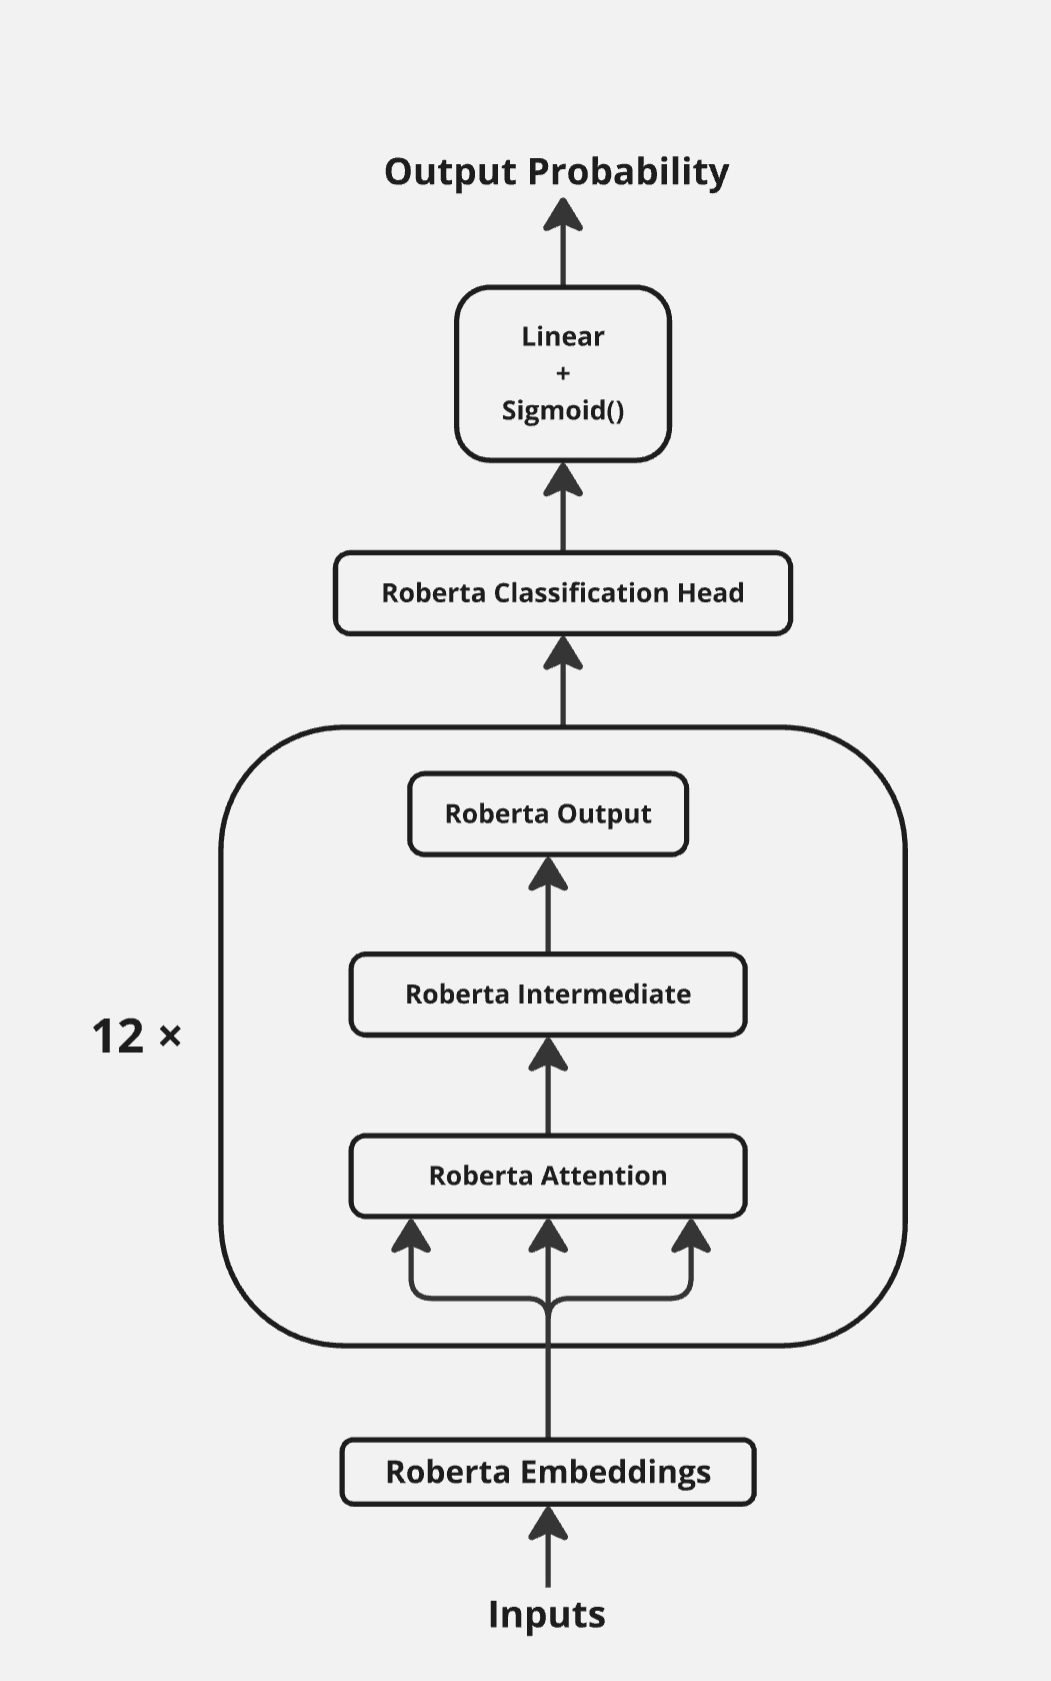
\includegraphics[width=\linewidth]{Images/Screenshot_20241023_113542_Miro.jpg}
        \caption{Original unitary/unbiased-toxic-roberta model}
        \label{fig:org-model}
    \end{subfigure}
    \hfill
    \begin{subfigure}[b]{0.45\linewidth} 
        \centering
        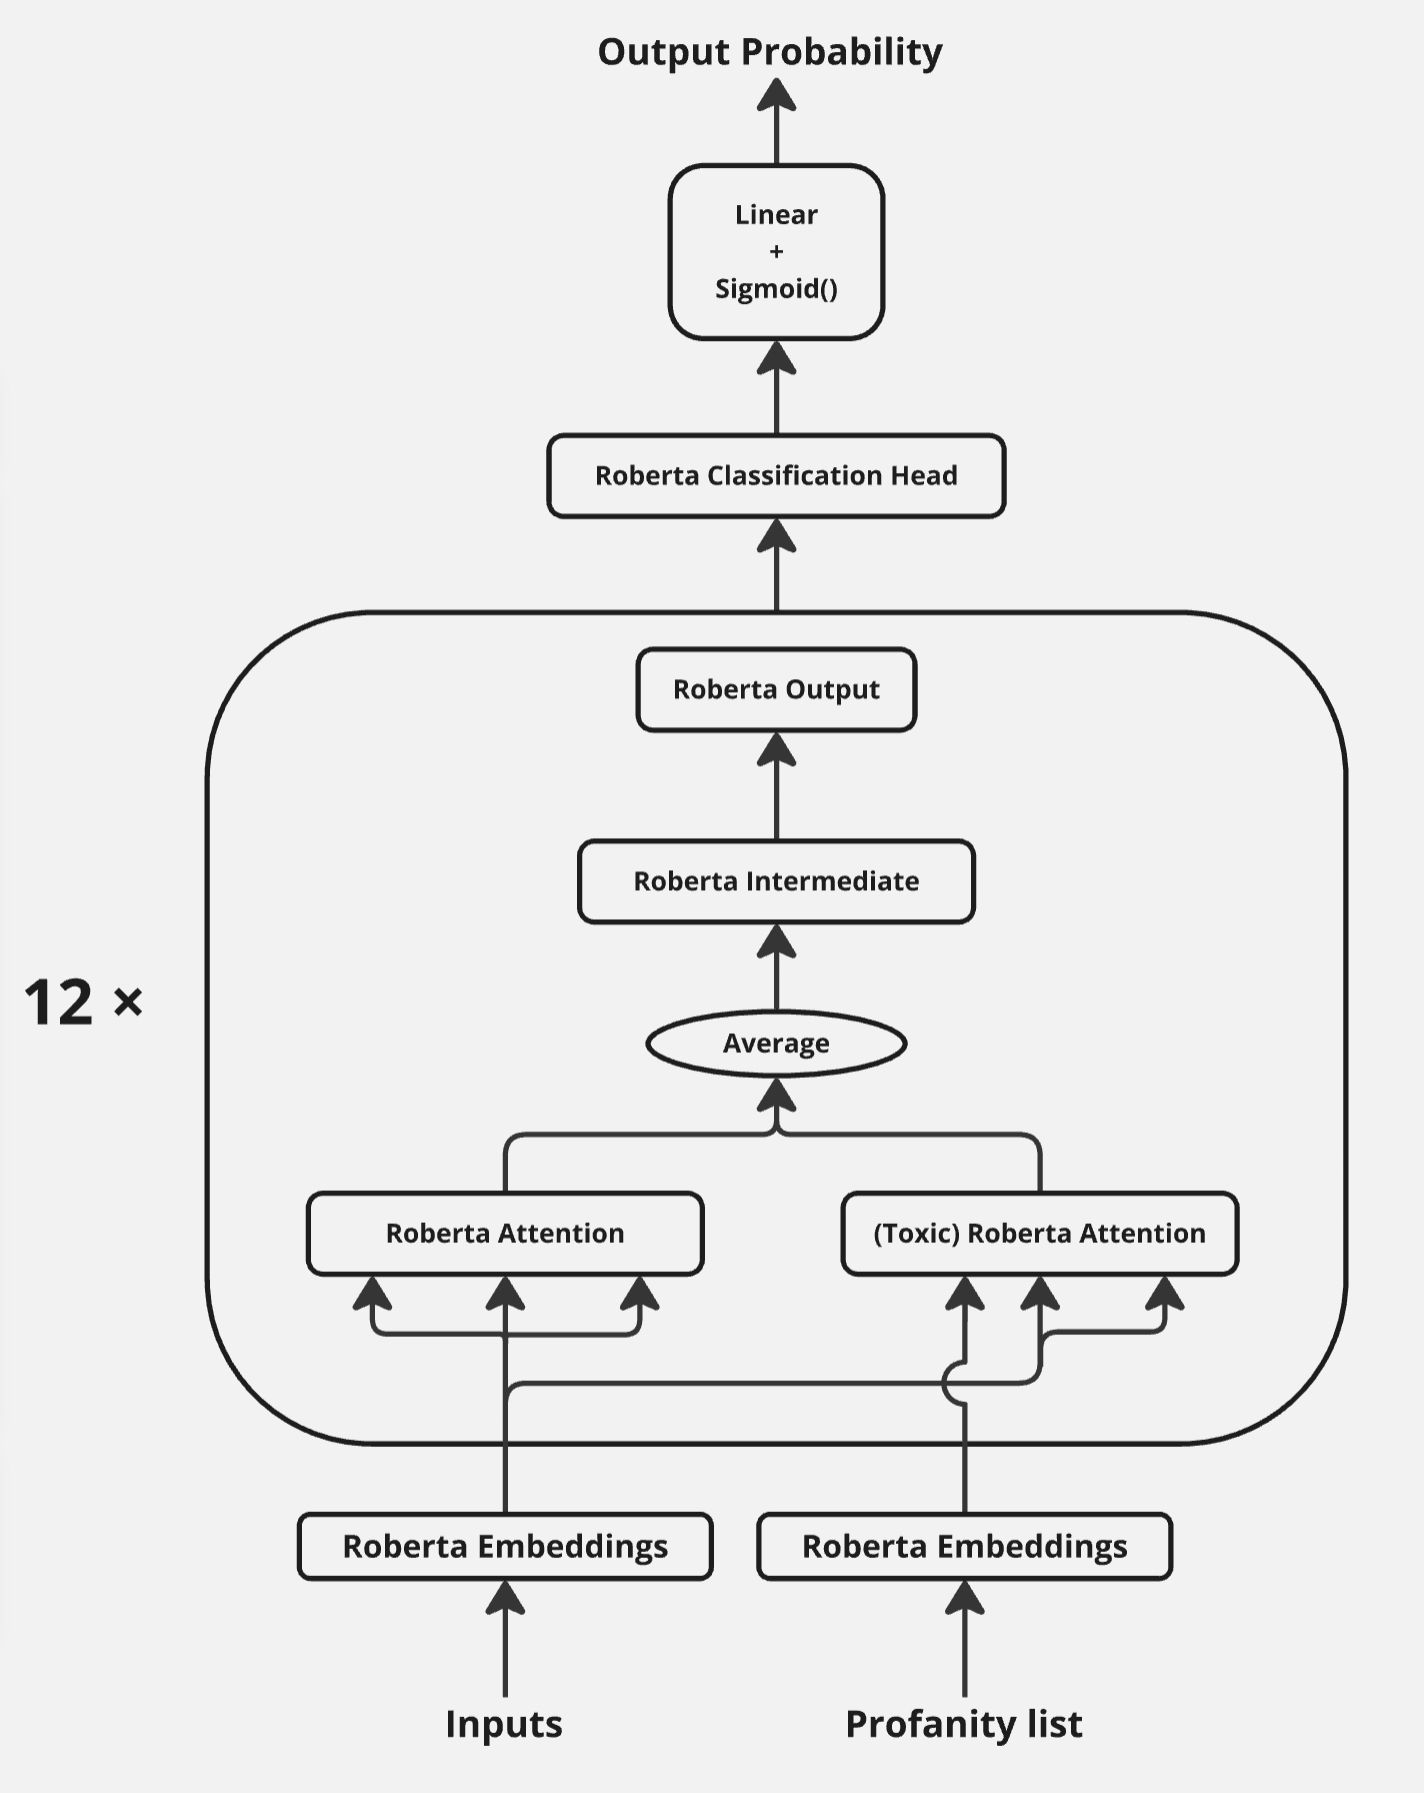
\includegraphics[width=\linewidth]{Images/Screenshot_20241023_113521_Miro.jpg}
        \caption{Toxic-attended roberta model}
        \label{fig:modified-model}
    \end{subfigure}
    
    \caption{Comparison between the original unitary/unbiased-toxic-roberta model and the modified Toxic-attended Roberta model}
    \label{fig:main-figure}
\end{figure}